\documentclass[11pt,a4paper]{article}
\usepackage[margin=2.2cm]{geometry}
\usepackage{graphicx}
\usepackage{enumitem}
\usepackage{titlesec}
\usepackage{xcolor}
\usepackage{parskip}
\usepackage{array}
\usepackage{hyperref}

\hypersetup{
  colorlinks=true,
  linkcolor=black,
  urlcolor=blue
}

\setlength{\parindent}{0pt}
\setlist[itemize]{leftmargin=1.5em}
\setlist[enumerate]{leftmargin=1.8em}

\definecolor{titlecolor}{RGB}{33,66,99}
\definecolor{rulecolor}{RGB}{180,180,180}

\titleformat{\section}
  {\Large\bfseries\color{titlecolor}}
  {\thesection.}
  {0.5em}
  {}

\titleformat{\subsection}
  {\large\bfseries}
  {}
  {0em}
  {}

\newcommand{\manualrule}{\vspace{0.5em}\hrule height 0.6pt \color{rulecolor}\vspace{0.8em}}

\begin{document}

\begin{center}
  {\LARGE\bfseries Estacion de Monitoreo de Suelo\par}
  \vspace{0.4em}
  {\large Manual de Uso en Terreno\par}
  \vspace{0.6em}
  {\normalsize Proyecto SUELO\_EC\_T\_HX2\par}
\end{center}

\manualrule

Este equipo mide condiciones del suelo y del ambiente, guarda los datos en una tarjeta SD y los envia automaticamente por red celular cuando hay cobertura.

El sistema esta pensado para operar de forma autonoma en terreno, con ciclos de medicion y suspension para reducir el consumo de energia.

\section{Que mide la estacion}

La estacion registra automaticamente:

\begin{itemize}
  \item Temperatura del aire
  \item Humedad del aire
  \item Temperatura del suelo
  \item Humedad del suelo
  \item Conductividad electrica del suelo
  \item Nivel de senal celular
  \item Voltaje de bateria
\end{itemize}

Si no hay cobertura celular, los datos no se pierden: quedan almacenados localmente y se envian cuando la comunicacion se recupera.

\section{Antes de instalar en terreno}

Verifique siempre lo siguiente:

\begin{itemize}
  \item La tarjeta SD esta insertada y operativa
  \item La SIM tiene plan de datos activo
  \item La bateria esta conectada o cargada
  \item Los sensores estan conectados
  \item La antena celular esta conectada
\end{itemize}

Si falta cualquiera de estos elementos, el sistema puede medir parcialmente o dejar de transmitir.

\section{Funcionamiento normal}

En operacion normal, el equipo:

\begin{enumerate}
  \item Despierta automaticamente
  \item Lee los sensores
  \item Guarda la medicion en la SD
  \item Intenta transmitir los datos
  \item Apaga perifericos y entra en suspension
\end{enumerate}

Este ciclo se repite cada \textbf{30 minutos}.

No requiere intervencion humana durante la operacion normal.

\section{Indicadores luminosos}

Las luces del equipo permiten diagnosticar rapidamente el estado de la estacion en terreno.

\subsection{Luz verde}

\begin{center}
  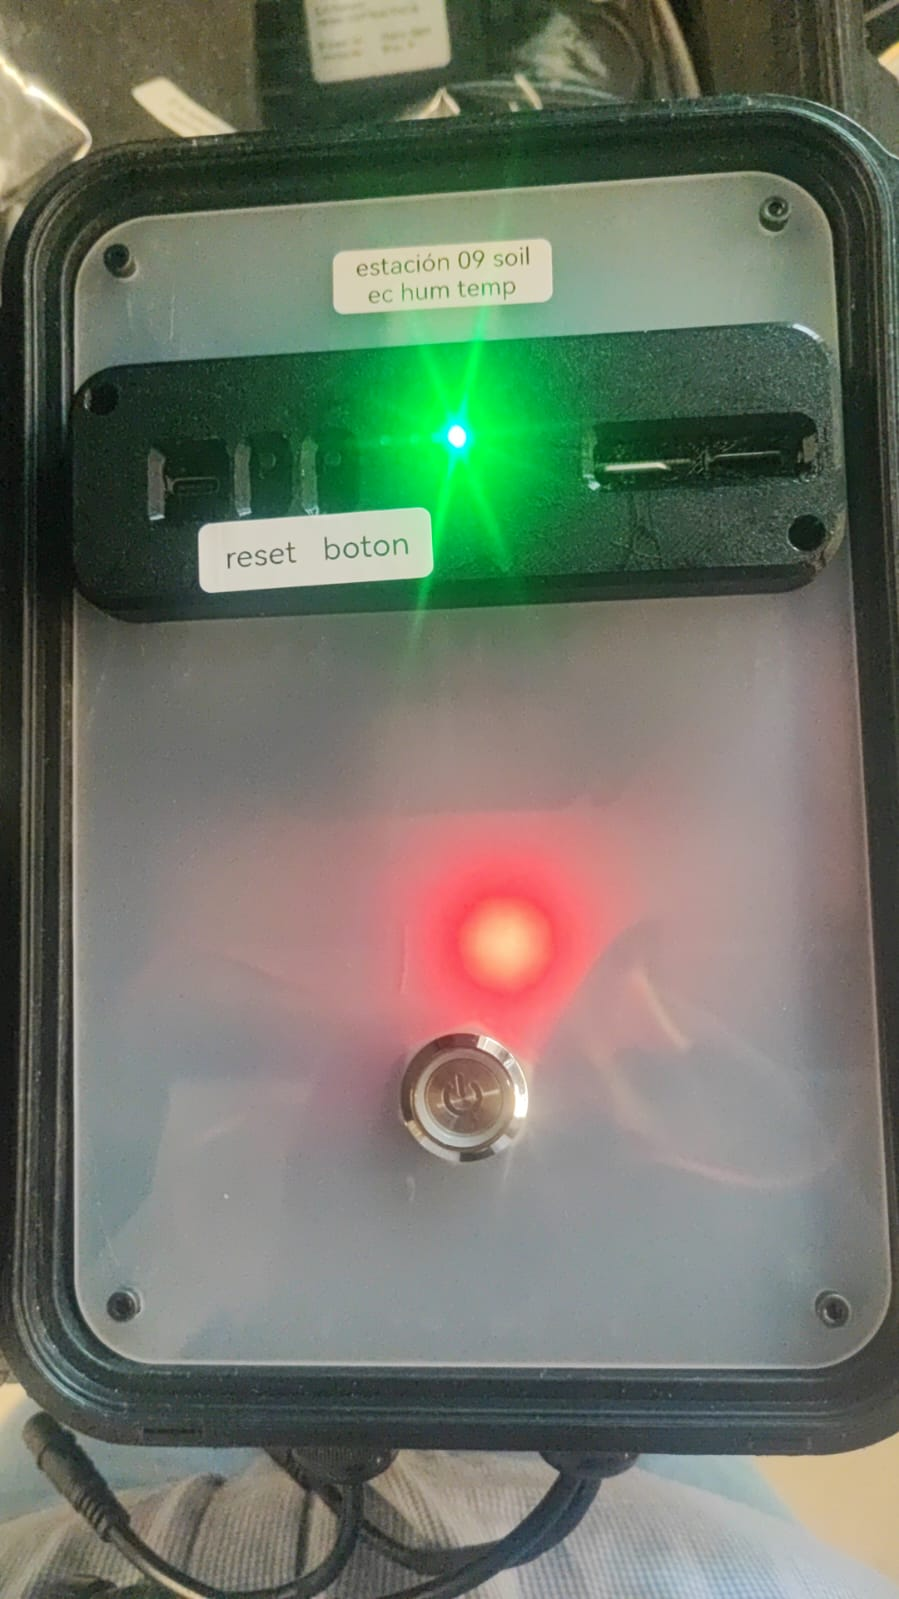
\includegraphics[width=0.28\textwidth]{luzverde.png}
\end{center}

Indica:

\begin{itemize}
  \item Medicion correcta
  \item Guardado correcto en la tarjeta SD
  \item Fin exitoso del ciclo de operacion
\end{itemize}

Si aparece de forma periodica, el equipo esta funcionando correctamente.

\subsection{Luz amarilla}

\begin{center}
  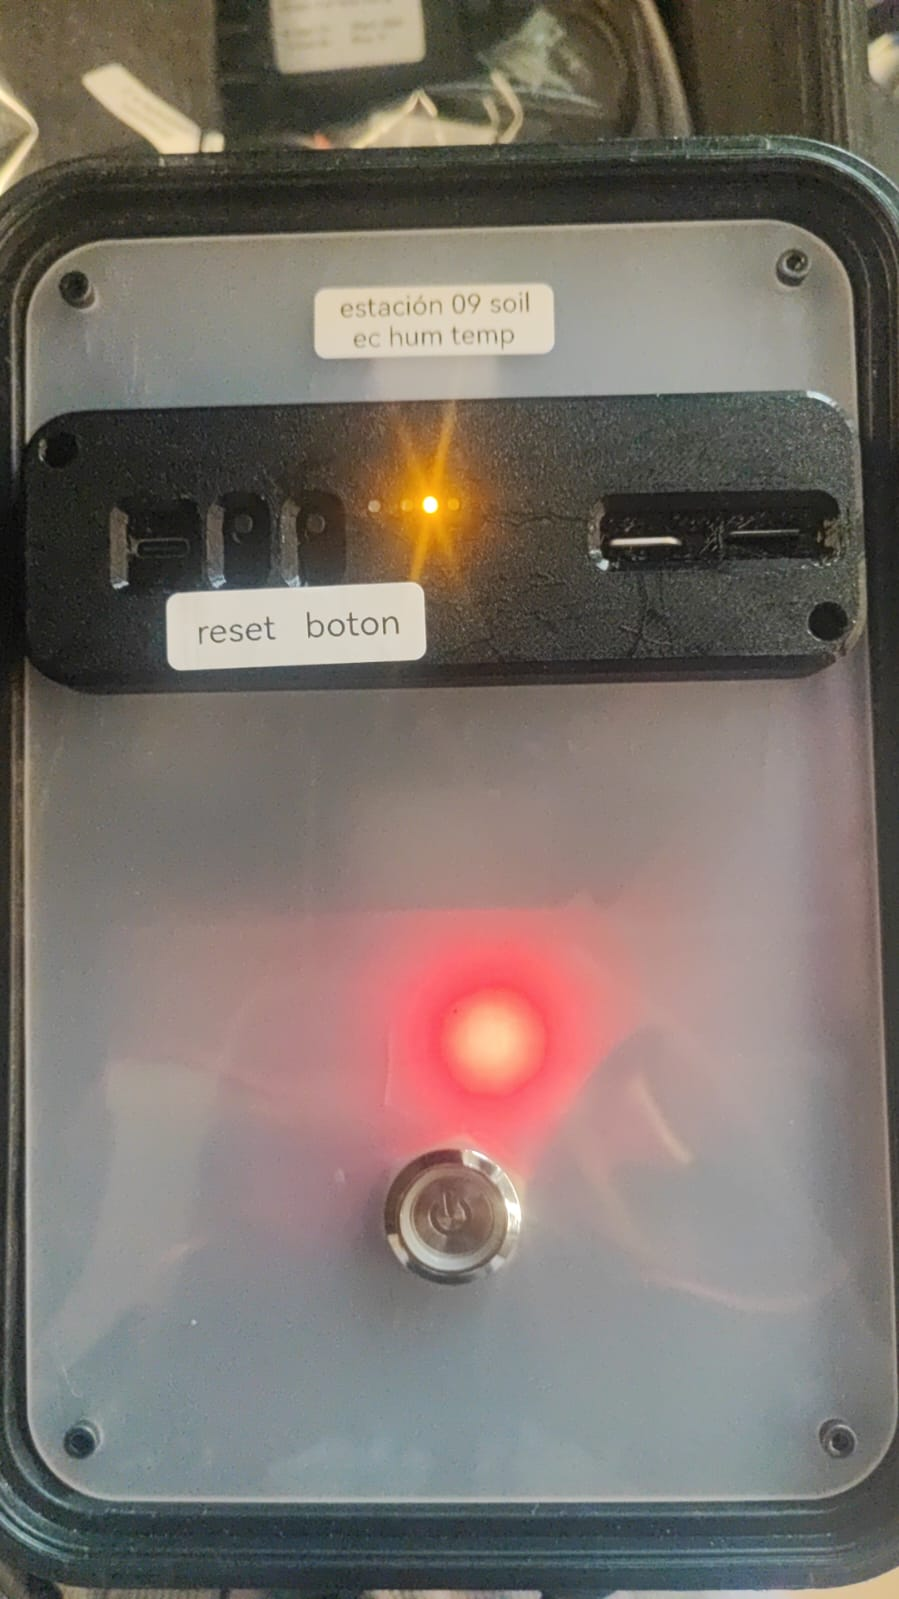
\includegraphics[width=0.28\textwidth]{luzamarilla.png}
\end{center}

Indica:

\begin{itemize}
  \item Transmision de datos en curso
  \item Modo burst activo
  \item Equipo ocupado en una tarea de mayor duracion
\end{itemize}

Si aparece durante algunos segundos, es normal.

\subsection{Luz roja}

Indica una condicion de error, normalmente asociada a almacenamiento o comunicacion.

Si aparece de forma persistente, revisar:

\begin{itemize}
  \item Tarjeta SD
  \item Senal celular
  \item Alimentacion del equipo
  \item Estado general de conexiones
\end{itemize}

\section{Que pasa si no hay senal celular}

No es una falla critica.

En esa condicion, el equipo:

\begin{itemize}
  \item Guarda todos los datos internamente
  \item Mantiene un cache de envio pendiente
  \item Reintenta la transmision en ciclos posteriores
\end{itemize}

No es necesario intervenir de inmediato si la estacion sigue midiendo y almacenando.

\section{Modo de medicion intensiva (modo burst)}

El equipo dispone de un modo especial para medicion intensiva.

Este modo sirve para:

\begin{itemize}
  \item Diagnostico en terreno
  \item Validacion tecnica
  \item Campanas de observacion de alta frecuencia
\end{itemize}

\subsection{Como activarlo}

\begin{enumerate}
  \item Energizar o despertar el equipo
  \item Presionar el boton \texttt{BOOT} en el momento de arranque o wakeup
  \item Verificar que el equipo entre al modo burst
\end{enumerate}

\subsection{Que hace el modo burst}

\begin{itemize}
  \item Realiza 36 lecturas
  \item Guarda una lectura cada 5 minutos
  \item Tiene una duracion total aproximada de 3 horas
  \item Almacena los datos en la SD
  \item Omite la transmision normal mientras el burst esta en ejecucion
\end{itemize}

Durante este modo, la luz amarilla actua como indicador de actividad.

\section{Almacenamiento de datos}

Los datos se guardan en la tarjeta SD en dos archivos principales:

\begin{itemize}
  \item \texttt{DATA[ID].CSV}: historial permanente de mediciones
  \item \texttt{cache.csv}: datos pendientes de transmision
\end{itemize}

Esto permite recuperar informacion incluso si:

\begin{itemize}
  \item No hubo senal durante varios dias
  \item El modem no pudo transmitir
  \item Hubo reinicios o fallas de red
\end{itemize}

\section{Consumo energetico}

El sistema esta disenado para bajo consumo.

Por eso:

\begin{itemize}
  \item Permanece dormido la mayor parte del tiempo
  \item Solo activa sensores, SD y modem cuando corresponde
  \item Apaga perifericos antes de volver a suspension
\end{itemize}

Esto es normal y forma parte del diseno del equipo.

\section{Cuando intervenir en terreno}

Se recomienda revisar el equipo si ocurre alguna de estas condiciones:

\begin{itemize}
  \item No hay luces durante varias horas
  \item La luz roja permanece encendida o aparece en todos los ciclos
  \item No hay datos reportados durante varios dias
  \item El equipo sufrio golpes, ingreso de agua o humedad extrema
  \item La antena o el cableado presentan danos visibles
\end{itemize}

\section{Recomendaciones de operacion}

Para una operacion confiable en terreno:

\begin{itemize}
  \item Mantenga la SD correctamente insertada
  \item Verifique periodicamente el estado de la bateria
  \item Evite desconectar antena o sensores con el equipo energizado
  \item Revise la cobertura celular del sitio de instalacion
  \item Inspeccione sellos, conectores y caja ante condiciones climaticas severas
\end{itemize}

\section{Responsabilidad operativa}

El correcto funcionamiento depende de:

\begin{itemize}
  \item Instalacion adecuada
  \item Estado de la bateria
  \item Cobertura celular
  \item Integridad de sensores, antena y tarjeta SD
  \item Condiciones ambientales del sitio
\end{itemize}

El sistema es autonomo, pero requiere supervision periodica.

\end{document}
